\documentclass[10pt,a4paper,onecolumn]{article}

\usepackage[utf8]{inputenx}
\usepackage[T1]{fontenc}
\usepackage{lmodern}
\usepackage{listings}
\usepackage{textcomp}
\usepackage[english,italian]{babel}
\usepackage{amsmath}
\usepackage{booktabs}
\usepackage{graphicx}
\usepackage[font=small,labelfont=bf,labelsep=period,tableposition=top]{caption}
\usepackage{tabularx}
\usepackage{multirow}
\usepackage{longtable}
\usepackage{fancyhdr}
\usepackage{lastpage}    
\usepackage{color}
\usepackage{enumitem}

\fancyhead{}
\renewcommand{\headrulewidth}{1pt}

\fancyhead[RE,RO]{
\begin{picture}(-135,0)
	\put(-475,0){\sffamily\large\leftmark}
\end{picture}
}

\cfoot{}

\fancyfoot[RO,LE]{\sffamily Pag.~\thepage{} di \pageref{LastPage}} 
\fancyfoot[RE,LO]{RistorESU Nord Piovego}

\renewcommand{\footrulewidth}{.2pt}
\pagestyle{fancy}

\renewcommand{\sectionmark}[1]{\markboth{#1}{#1}} 

% **************************************************
% Cross-references e collegamenti ipertestuali
% **************************************************
\usepackage[]{hyperref}
%\usepackage[hidelinks]{hyperref}
\hypersetup{%
  colorlinks=false, linktocpage=false, pdfborder={0,0,0}, pdfstartpage=1, pdfstartview=FitV,%
  urlcolor=Cyan, linkcolor=Cyan, citecolor=Black, %pagecolor=Black,
  pdfcreator={pdflatex}, pdfproducer={pdflatex with hyperref package}%
}

\definecolor{dkgreen}{rgb}{0,0.6,0}
\definecolor{gray}{rgb}{0.5,0.5,0.5}
\definecolor{mauve}{rgb}{0.58,0,0.82}
 
\lstset{ %
  %language=XHTML,                % the language of the code
  basicstyle=\footnotesize,           % the size of the fonts that are used for the code
  numbers=left,                   % where to put the line-numbers
  numberstyle=\tiny\color{gray},  % the style that is used for the line-numbers
  stepnumber=2,                   % the step between two line-numbers. If it's 1, each line 
                                  % will be numbered
  numbersep=5pt,                  % how far the line-numbers are from the code
  backgroundcolor=\color{white},      % choose the background color. You must add \usepackage{color}
  showspaces=false,               % show spaces adding particular underscores
  showstringspaces=false,         % underline spaces within strings
  showtabs=false,                 % show tabs within strings adding particular underscores
  frame=single,                   % adds a frame around the code
  rulecolor=\color{black},        % if not set, the frame-color may be changed on line-breaks within not-black text (e.g. comments (green here))
  tabsize=2,                      % sets default tabsize to 2 spaces
  captionpos=b,                   % sets the caption-position to bottom
  breaklines=true,                % sets automatic line breaking
  breakatwhitespace=false,        % sets if automatic breaks should only happen at whitespace
  title=\lstname,                   % show the filename of files included with \lstinputlisting;
                                  % also try caption instead of title
  keywordstyle=\color{blue},          % keyword style
  commentstyle=\color{dkgreen},       % comment style
  stringstyle=\color{mauve},         % string literal style
  escapeinside={\%*}{*)},            % if you want to add LaTeX within your code
  morekeywords={*,...},              % if you want to add more keywords to the set
  deletekeywords={...}              % if you want to delete keywords from the given language
}

% **************************************************
% Macro
% **************************************************
\newcommand{\sitepage}[1]{\textcolor{cyan}{\textsf{#1}}}
\newcommand{\inglese}[1]{\foreignlanguage{english}{\itshape{}#1}}
\newcommand{\progname}[1]{\textcolor{blue}{\textsf{#1}}}

\begin{document}
%----------------------------------------------------------
\begin{titlepage}

\begin{center}
% Upper part of the page
 
\textsc{\Large}\\[5cm]


\includegraphics[width=0.4\textwidth]{Logo.png}\\[0.3cm]  
\noindent\rule{\textwidth}{0.4pt} \\[0.3cm]
\textsc{\Huge Progetto di}\\[0.25cm]
\textsc{\Huge Tecnologie Web}\\[0.3cm]
\textsc{\Large Sito ``RistorESU Nord Piovego''}
\noindent\rule{\textwidth}{0.4pt}\\[0.5cm]
\textit{``Sviluppare un sito secondo gli standard W3C e le direttive WCAG 2 AAA''} \\[0.5cm]
\textsc{23 febbraio 2014}\\[0.5cm]
\begin{minipage}{0.4\textwidth}
\begin{flushleft} \large
\emph{Studente:}\\
Claudio Guarisco\\
Daniele Ronzani\\
Gianluca Bariga Boscolo\\
Michele Massaro
\end{flushleft}
\end{minipage}
\begin{minipage}{0.4\textwidth}
\begin{flushright} \large
\emph{Matricola:} \\
1057761\\
1057310\\
1061301\\
1057513\\
\end{flushright}
\end{minipage}
\end{center}
\end{titlepage}
%-----------------------------------------------------------------------

\clearpage

\tableofcontents

\clearpage 

\begin{abstract}
Questo progetto consiste nella realizzazione di un sito per la mensa 'RistorESU Nord Piovego'.
Si tratta di un sito che permette di ottenere informazioni utili per tutti gli utilizzatori del servizio di ristorazione della mensa Piovego, come ad esempio la lista dei piatti serviti, le informazioni sulle tariffe o la posizione geografica.
\end{abstract}

\clearpage

\section{Analisi dei requisiti}
Il sito è stato progettato per avere come target gli studenti universitari, che rappresentano la maggior parte degli utilizzatori del servizio di ristorazione della mensa Piovego. Inoltre si è cercato di capire quali informazioni siano di maggior interesse, in modo da renderle semplici e veloci da reperire.
Dato che nel nostro bacino di potenziali utenti sono presenti anche molti studenti provenienti da altre nazioni, e quindi con difficoltà nel comprendere l'italiano, abbiamo pensato di tradurre ogni pagina del sito anche in lingua inglese in modo da rendere possibile la fruizione dei contenuti anche per loro. \\
Dato che è un sito in cui la maggior parte degli utilizzatori è in età giovanile, si è cercato di utilizzare una grafica semplice e colorata. Il colore principale (giallo) è stato scelto per richiamare gli elementi cromatici presenti nella sede fisica della mensa, in modo da rendere coerente il sito con ciò che rappresenta.

\section{Design}

\subsection{Layout}

Il layout consiste quasi completamente in una classica disposizione a tre pannelli, in cui possiamo trovare in ogni pagina i seguenti elementi:

\begin{figure}[h]
\centering
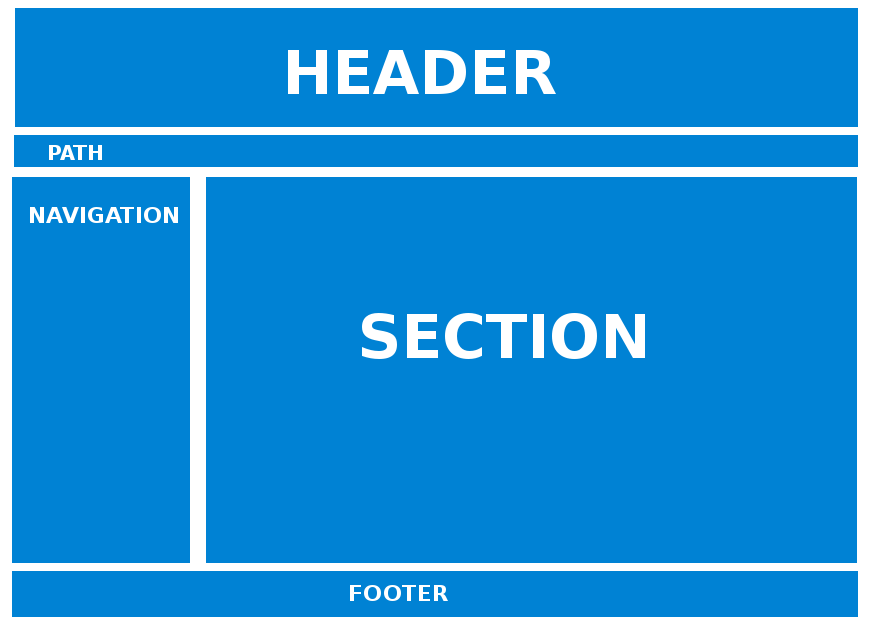
\includegraphics[scale=0.25]{layout}
\caption{Layout utilizzato dal sito}
\label{layoutPic}
\end{figure}

\begin{itemize}
 \item \textbf{Header}: parte superiore che contiene il titolo della pagina e l'indicazione della lingua.
 \item \textbf{Path}: sezione immediatamente sottostante all'header in cui viene indicata la posizione attuale assoluta all'interno del sito.
 \item \textbf{Navigation}: la parte sinistra di ogni pagina è occupata dal menù di navigazione, che contiene i link per le pagine principali.
 \item \textbf{Section}: la parte a destra del menù contiene il vero contenuto, ovvero la parte variabile che cambia per ogni pagina.
 \item \textbf{Footer}: la parte inferiore del sito contiene le informazioni accessorie, dato che è quella meno visibile per l'utente; in questo caso contiene i link ai social network, il nome team che ha realizzato il sito e le certificazioni W3C.
\end{itemize}

Per garantire una corretta visualizzazione tramite ogni dispositivo si è scelto di utilizzare un layout elastico, che permette il ridimensionamento negli schermi dei PC ma arriva ad un punto di rottura che cambia completamente la presentazione nel caso di larghezza del display troppo piccolo. In questo modo si riesce a sfruttare al meglio le diverse dimensioni, permettendone l'utilizzo sia da PC che da dispositivi mobile.
La completa divisione tra contenuto e presentazione ha reso più facile questa operazione, dato che in questo modo non è stato necessario mobificare il contenuto HTML delle pagine, ma solo il CSS.
In totale sono stati usati tre layout CSS differenti:
\begin{itemize}
 \item il principale (\textit{style.css}) contiene la presentazione per schermi medio grandi, contenente la disposizione vista precedentemente;
 \item la versione mobile per schermi piccoli (\textit{small.css}), in cui la disposizione è stata studiata per permetterne l'utilizzo tramite touchscreen, e quindi contiene bottoni più grandi ed uno stile più verticale "scroll-friendly";
 \item l'ultimo è il layout per la stampa (\textit{print.css}), che rimuove gli elementi che non necessitano di essere stampati (come il menù) ed utilizza un font più consono per la carta stampata (\textit{Times New Roman}).
\end{itemize}

\begin{figure}[h]
\centering
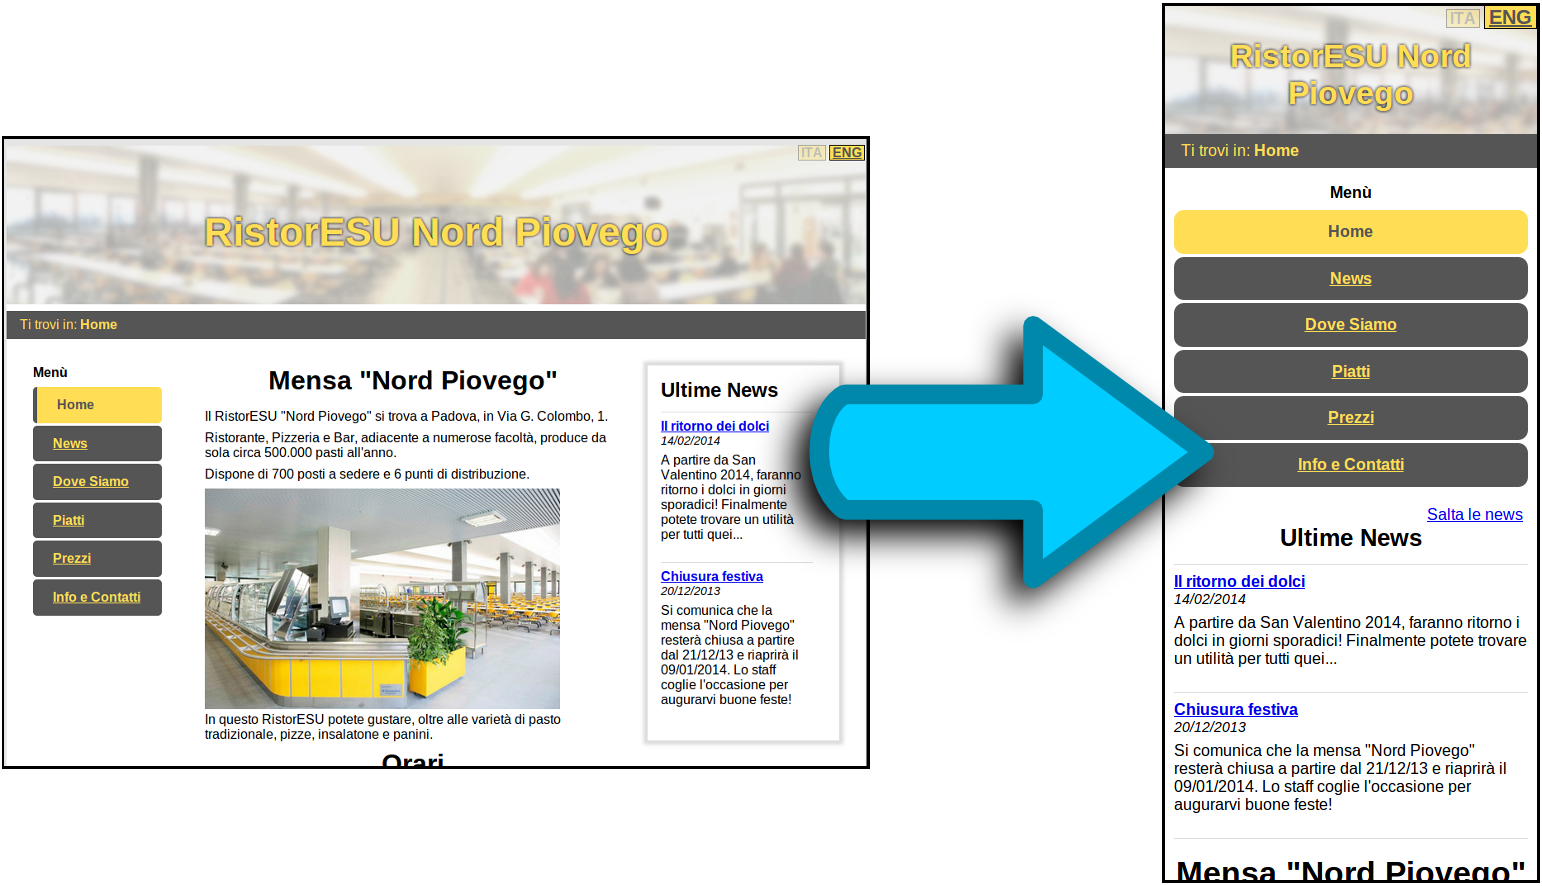
\includegraphics[scale=0.20]{trasformazione}
\caption{Layout normale e mobile}
\label{trasformazioneMobile}
\end{figure}

Inoltre, all'interno di ogni foglio di stile le dimensioni di tutti gli elementi sono state definite tramite percentuali (nel caso di posizionamenti) o "em" (nel caso di grandezza del testo), in modo che la pagina si adatti ad ogni tipo di schermo.
Per migliorare il supporto ai diversi sistemi operativi sono state definite più famiglie di font, in modo che l'assenza di supporto per uno specifico font non causi un fallback su un altro non adatto per il sito; in particolare, l'ordine di font family è \textit{Helvetica}, \textit{Arial} e \textit{sans-serif}.

\subsection{Struttura organizzativa}

La struttura organizzativa utilizzata dal sito è gerarchica, ed è stata scelta per permettere all'utente di orientarsi facilmente. A tale scopo è stata mantenuta una profondità media molto bassa, mantenendo anche una ridotta ampiezza utilizzando solo sei voci nel menù, in modo che l'utente possa facilmente creare una propria mappa mentale e evitare il disorientamento.
Inolte si è cercato di mantenere sempre presenti alcune informazioni importanti, che permettano di rispondere alle principali informazioni di cui l'utente ha bisogno. Per farlo è stato controllato che le sei domande principali rappresentate dai sei assi W fossero risposte nell'home page, come ad esempio ``Di cosa parla il sito?'', ``Cosa offre il sito?'', o ``Come raggiungere le sezioni principali del sito?''.

\section{Dati}

I dati del sito sono salvati in un database XML, per cui è stato definito un XMLSchema che propone la struttura visibile nella Figura \ref{xml}. È stato usato il modello di progettazione ``tende alla veneziana'', in modo da garantire la possibilità di riutilizzo dei tipi avendo solo un elemento globale. 
È stato deciso di utilizzare un solo database per tutto il sito, utilizzando di volta in volta solo alcune informazioni durante la generazione delle pagine; questa scelta è stata dettata dal fatto che tutti i dati inseriti sono logicamente correlati tra loro.
Considerando che l'elaborazione viene effettuata server side, non è presente il problema dello spreco di banda per l'invio della totalità delle informazioni, poichè al client vengono inviate solo le informazioni effettivamente visualizzate.
La radice ``piatti'' rappresenta quale tipologia di dati vogliamo salvare, cioè le informazioni relative alle portate disponibili.
Gli altri elementi importanti sono:
\begin{itemize}
 \item \textbf{Piatto}: rappresenta il singolo piatto, e contiene le informazioni principali, quali il nome, la descrizione e l'immagine (come path). Inoltre tutte le informazioni contenenti testo sono state aggiunte due volte utilizzando un suffisso diverso per il nome dell'elemento: uno per la lingua italiana e uno per la lingua inglese.
 \item \textbf{Commento}: ogni piatto contiene un figlio ``\textit{commenti}'', che a sua volta può contenere molti figli ``\textit{commento}'', che possiedono tutte le informazioni relative ad un singolo commento, come la data, l'autore, il testo e la lingua utilizzata dall'utente durante la scrittura.
\end{itemize}
Come detto precedentemente, pagine diverse utilizzano diversi elementi del database, in particolare:
\begin{itemize}
 \item il foglio di trasformazione piatti.xsl utilizza gli elementi ``\textit{piatto}'' per costruire dinamicamente la lista delle portate disponibili;
 \item il foglio viewpiatto.xsl utilizza l'elemento ``\textit{piatto}'' e le sue informazioni per costruire un resoconto dettagliato di una singola portata, includendo anche la visualizzazione dei commenti.
\end{itemize}
L'utilizzo specifico verrà trattato successivamente all'interno della descrizione delle singole pagine.

\begin{figure}[h]
\centering
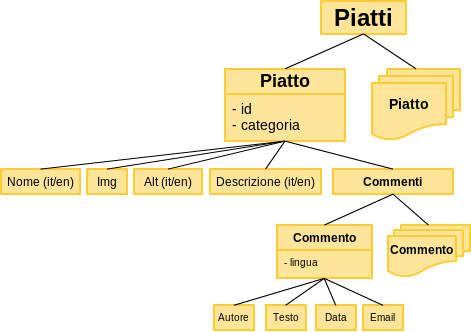
\includegraphics[scale=0.55]{alberoXML}
\caption{Struttura del file piatti.xml}
\label{xml}
\end{figure}

\section{Analisi generale dell'accessibilità}

Riguardo l'accessibilità si è scelto di rispettare le direttive WCAG 2 AAA, e alcune delle scelte più importanti verranno descritte di seguito.

\subsubsection{Colori}

Come anticipato precedentemente, la scelta cromatica è stata fatta in base ai colori che rappresentano al meglio la mensa Piovego. Prima di applicare i vari colori al sito, è stato controllato che mantenessero sempre un contrasto molto alto, in modo da non creare alcun problema di accessibilità a persone con disturbi visivi. Inoltre in tutto il sito non sono mai state veicolate informazioni tramite colori, per evitare che gli utenti ipovedenti, o con problemi di daltonismo, non riescano ad accedervi. Un esempio è la barra nera presente a fianco dell'elemento del menù selezionato, in modo che l'informazione sulla pagina corrente sia più evidente. \\
Per l'analisi in caso di daltonismo ci siamo affidati al sito \textit{http://vischeck.com/}, e i risultati sono evidenti dalla Figura \ref{colors}. Si puà notare che i contenuti sono comprensibili anche nel caso più raro di tritanopia. \\

\begin{figure}[h]
\centering
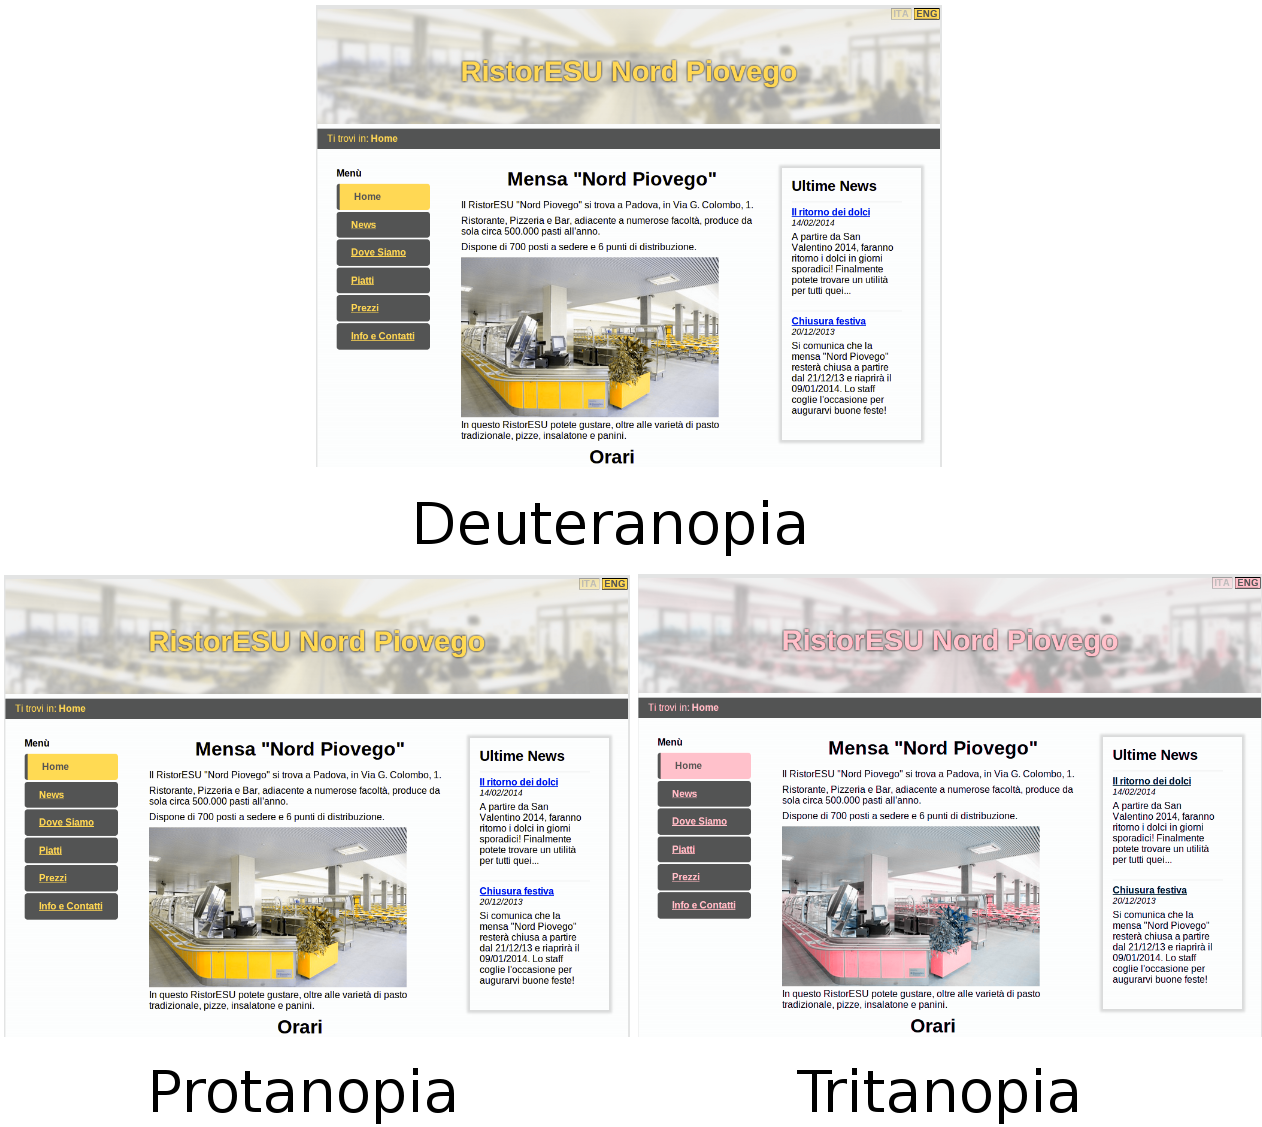
\includegraphics[scale=0.25]{home_colors}
\caption{Come viene vista l'home page in caso di daltonismo}
\label{colors}
\end{figure}

\subsubsection{Testo}

Dire che il testo \'e sempre diviso in sezioni per favorire la lettura

\subsubsection{Immagini}

\subsubsection{Link}

Sono sempre sottolineati e il colore varia per quelli visitati

\subsubsection{Screen Reader}

escono i link e la disposizione \'e bella (parlare anche dei test)

\clearpage
\section{Mappa del sito}

\includegraphics[width=.9\textwidth]{mappasito.png}


\clearpage

\section{Pagine significative}

Verranno ora descritte le tecniche scelte ed utilizzate nella costruzione delle pagine con caratteristiche diverse rispetto al resto del sito.

\subsection{Index}

TODO parlarne un po'

\subsubsection{Disposizione}

TODO Dire che abbiamo dovuto mettere le news prima della section altrimenti non funzionava. Dire anche che i link delle news hanno le ancore su ogni news.

\subsubsection{Javascript}

\subsection{Dove Siamo}

TODO parlarne un po'

\subsubsection{Mappa}

TODO dire come abbiamo sostituito l'immagine e perche'

\subsection{Piatti}

TODO parlarne un po'

\subsubsection{Creazione dinamica}

TODO parlare ampiamente del cgi e xsl

\subsection{Viewpiatto}

TODO parlarne un po'

\subsubsection{Creazione dinamica}

TODO parlare ampiamente del cgi e xsl

\subsubsection{Form}

TODO parlare ampiamente del form e dei controlli JS e Perl

\clearpage

\section{Test}

TODO parlare dei test effettuati, sui browser, screenreader, lynx, ... e delle validazioni.

\section{Conclusioni}

TODO boh, possiamo anche toglierle

\end{document}


